\documentclass[a4paper, 12pt]{article}
\usepackage[utf8]{inputenc}
\usepackage[portuguese]{babel}

\usepackage{mathptmx}
\usepackage{enumitem}
\usepackage{amsmath}

% Margins
\usepackage{geometry}
\geometry{left=30mm,right=20mm,%
bindingoffset=0mm, top=30mm,bottom=20mm,includefoot}

% Images
\usepackage{graphicx}
\graphicspath{ {./images/} }

% Title font size
\usepackage{titlesec}
\titleformat*{\section}{\bfseries}

% Indent first sentence of a paragraph
\usepackage{indentfirst}

% highlight code
\usepackage{listings}

% Page numbers at bottom right
\usepackage{fancyhdr}
\pagestyle{fancy}
\fancyhf{}
\renewcommand{\headrulewidth}{0pt}
\rfoot{\thepage}

% 1.5 line spacing (yes, 1.25 is actually 1.5)
\fontsize{10}{12}
\linespread{1.50}
\fontfamily{ptm}
\selectfont

% Fix vspacing for section titles
\let\oldsection\section
\renewcommand{\section}[1]{{\vspace{20pt}\oldsection*{#1}\vspace{-10pt}}}

% Indent size
\setlength\parindent{10mm}

% Jump 20pt
\newcommand{\jump}[1]{{\vspace{20pt}}}

\newenvironment{leftquote}[1][]
{
    \hspace{30pt} #1
    \vspace{20pt}
    \fontsize{10}{10}\selectfont
    \begin{flushright}
    \begin{minipage}{120mm}
}
{
    \end{minipage}
    \end{flushright}
    \par
    \vspace{20pt}
}

\newcommand{\tmp}{}

\newenvironment{container}[3]
{
    \renewcommand{\tmp}{#3} %gambiarra
    
    \begin{center}
    \begin{minipage}{#1}
    \centering
    #2
}
{
    \raggedright
    {\footnotesize \tmp}
    \end{minipage}
    \end{center}
}

\begin{document}

% Remove page number
\clearpage
\thispagestyle{empty}

\begin{bfseries}
\begin{center}


\includegraphics[scale=0.45]{ufc.png} \\
\vspace{-4pt} 
UNIVERSIDADE FEDERAL DO CEARÁ \\
\vspace{4pt} 
CENTRO DE TECNOLOGIA \\
\vspace{4pt} 
DEPARTAMENTO DE TELEINFORMÁTICA \\
\vspace{4pt}
a
\vspace{4pt}
SEMESTRE 2025.1 \\


\vspace*{\fill}
\textbf{Relatório dos Homeworks de Álgebra Linear e Multilinear}
\vspace*{\fill}

\end{center}

\begin{itemize}[leftmargin=*]
    \setlength{\itemsep}{0pt}
    \item[] ALUNO: Ruan Pereira Alves
    \item[] MATRÍCULA: 569551
\end{itemize}

\end{bfseries}
\newpage

\section{Homework 01}

Em álgebra linear, podemos verificar como podemos fazer a resolução de sistemas lineares de forma um pouco mais dinâmica, e especialmente como é possível realizar operações utilizando vetores coluna, o que permite interpretar as operações utilizando as colunas do sistema, mantendo o formato $Ax = b$. 

Um espaço vetorial é constituído de vetores que possuem as operações de adição de vetores e multiplicação de escalares, e que alguns axiomas devem ser seguidos para que as operações ocorram. O maior exemplo de um espaço vetorial é o espaço $R^n$, que pode possuir $n$ dimensões.

Um subespaço seria apenas um subconjunto de vetores dentro de um espaço vetorial, vide exemplo $R^3$.

Após isso, precisamos verificar se um dado conjunto de vetores possui independência linear, ou seja se os vetores só possuem uma forma de serem zerados, sendo "forçados" a serem zero. Em outras palavras, o espaço nulo da matriz A com os vetores só possui o vetor zero.

Com essa independência, podemos assim gerar um espaço com base no conjunto de vetores, em que as combinações destes vetores criam o espaço vetorial, ou seja baseado em operações entre esses vetores. O espaço vai consistir de todas as possíveis combinações lineares do conjunto de vetores. 

Uma base seria uma sequência de vetores que justamente possui as duas propriedades mencionadas acima. Para qualquer espaço, o número de vetores-base é uma propriedade do próprio espaço, ou seja para qualquer número de vetores-base de um espaço, o mesmo número de vetores é contido dentro do espaço, o que nos traz o conceito de dimensão. 

Para a verificação de um vetor arbitrário em um subespaço definido, é necessário realizar as operações vetoriais com os vetores-base do subespaço, buscando montar o vetor arbitrário a partir dos vetores-base, ou seja criando um sistema linear e o resolvendo. Se houver solução, o vetor pertence. 

Assim, foi possível realizar o desenvolvimento da atividade, vide o código a seguir: 

\begin{lstlisting}
	#include <iostream>
	#include <armadillo>
	
	using namespace std;
	using namespace arma;
	
	int main () {
		mat A = {{1,2,3},
			{4,5,6},
			{7,8,9}};
		
		cout << "hello" << A << endl;
		double det_A = det(A);
		cout << "det A = " << det_A << endl;
		mat B = {{3,2,1}, {0,0,0}, {0,0,0}};
		cout << A + B << endl;
		
		mat C = A * 2;
		cout << C << endl; 
		uword r = arma::rank(A);
		cout << r << endl;
		
		mat base = {{1,0,0}, {0,1,0},{0,0,1}};
		vector<double> arb = {2,2,1};
		
		return 0;
	}
	
\end{lstlisting}

\section{Homework 02 linear}

gomennasai
\section{Homework 03 linear}

yamete

\jump

A seguir, têm-se os exemplos de como fazer citações e referências.

\jump

Para Siss (2012) as políticas de ação afirmativas constituem políticas públicas, estatais e de caráter compulsório, elaboradas e implementadas pelo Estado, ou seja, é o Estado em ação.

Segundo Bastos e Keller (2006, p. 38), “A leitura é um processo que envolve algumas habilidades, entre as quais a interpretação do texto e a sua compreensão.”

As organizações testemunharam uma redução da validade de seu conhecimento durante este período e começaram a perceber que já não era possível confiar em Instituições de Ensino Superior para desenvolver a sua mão de obra (TARAPANOFF, 2006).

O discurso jurídico, que hoje se apresenta com um novo perfil, dispõe de um acervo variado de opções para ser construído, pois, “[...] agrega valores, impõe condutas, conduz instituições, movimenta riquezas, opta por visões de mundo e, portanto, sustenta uma ideologia.” (BITTAR, 2001, p. 181).


\jump

As ilustrações (fotografias, gráficos, mapas, plantas, quadros) e tabelas devem ser citados e inseridos o mais próximo possível do trecho a que se referem.

\jump

% http://pgfplots.net/tikz/examples/bar-plot/ (the "right" way to do it)
\begin{container}{10cm}{Gráfico 1 – Distribuição dos documentos analisados por programa de pós-graduação}{Fonte: Elaborado pelo autor.}

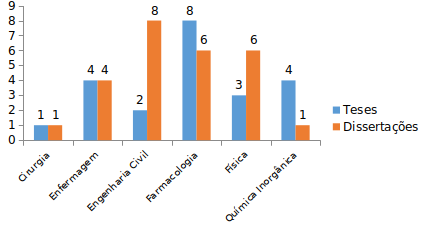
\includegraphics[width=10cm]{graph.png}

\end{container}

\begin{container}{10cm}{Figura 1 – Organização do conhecimento/Representação do
conhecimento, Organização da informação/Representação da informação}{Fonte: Lara e Smit (2010, com adaptações).}

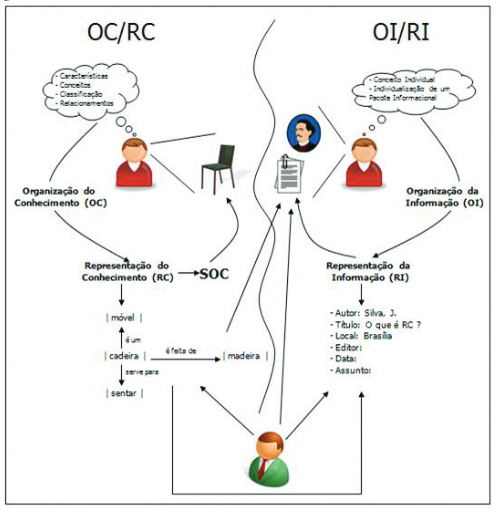
\includegraphics[width=10cm]{image.png}

\end{container}

\jump

\begin{container}{10cm}{Tabela 1 – Distribuição dos documentos analisados por programa de pós-graduação}{Fonte: elaborada pelo autor.}
\begin{center}
\begin{tabular}{ | c | c | c | c | }
    \hline
    Programas de pós-graduação & Teses & Dissertações & Total\\
    \hline
    \hline
    Cirurgia & 1 & 1 & 2 \\
    \hline
    Enfermagem & 4 & 4 & 8 \\
    \hline
    Engenharia Civil & 2 & 8 & 10 \\
    \hline
    Farmacologia & 8 & 6 & 14 \\
    \hline
    Física & 3 & 6 & 9 \\
    \hline
    Química Inorgânica & 4 & 1 & 5 \\
    \hline
    Total & 22 & 26 & 48 \\
    \hline
\end{tabular} 
\end{center}
\end{container}

\section{PROCEDIMENTO}
Nesta parte o aluno deve descrever detalhadamente os procedimentos realizados (em primeira pessoa); apresentar os resultados das medidas (tabelas, gráficos, cálculos, etc). Atenção: anotar sempre as unidades.


\section{QUESTIONÁRIO}
No questionário devem constar as perguntas e as respostas de acordo com o roteiro de prática do ano em curso. 


\section{CONCLUSÃO}
Parte final do texto na qual se apresentam as conclusões apoiadas no desenvolvimento do assunto. É a recapitulação sintética dos resultados obtidos. 

Na conclusão o aluno deve apresentar uma discussão sobre os resultados obtidos em função dos objetivos do experimento. Cabe também comentar sobre as possíveis fontes de erros.

\newpage

\begin{center}
    \textbf{REFERÊNCIAS}
\end{center}

\jump

{\parindent0pt % disables indentation for all the text between { and }

BASTOS, Cleverson Leite; KELLER, Vicente. \textbf{Aprendendo a aprender}: introdução à metodologia científica. 19. ed. Petrópolis: Vozes, 2006.

\jump

BITTAR, Eduardo Carlos Bianca. \textbf{Linguagem jurídica.} São Paulo: Saraiva, 2001.

\jump

LARA, Marilda Lopes Ginez de; SMIT, Johanna Wilhelmina. \textbf{Temas de pesquisa em Ciência da Informação no Brasil.} São Paulo: Escola de Comunicações e Artes da Universidade de São Paulo, 2010. Disponível em:
http://www.repositoriobib.ufc.br/000005/00000588.pdf. Acesso em: 21 jan. 2012.

\jump

MUELLER, Suzana Pinheiro Machado; PERUCCHI, Valmira. Universidades e a produção de patentes: tópicos de interesse para o estudioso da informação tecnológica. \textbf{Perspectivas em Ciência da Informação}, Belo Horizonte, v. 19, n. 2, p. 15-36, 2014.

\jump

SISS, Ahyas. Afro-brasileiros e Educação Superior: notas para debates. In: COSTA, Hilton; PINHEL, André; SILVEIRA, Marcos Silva da (org.). \textbf{Uma década de políticas afirmativas}: panorama, argumentos e resultados. Ponta Grossa: Editora UEPG, 2012. p. 18-26.

\jump

TARAPANOFF, K. Educação corporativa. In: CONGRESSO IBEROAMERICANO DE
GESTÃO DO CONHECIMENTO E INTELIGÊNCIA COMPETITIVA, 1., 2006, Curitiba.
\textbf{Anais} [...]. Curitiba: CIETEP, 2006. Disponível em: http://www.gecic.com.br. Acesso em: 22 out. 2006. p. 59-70.

\jump

UNIVERSIDADE FEDERAL DO CEARÁ. Biblioteca Universitária. \textbf{Guia de normalização de trabalhos acadêmicos da Universidade Federal do Ceará}. Fortaleza, 2013.

}

\end{document}
